\section{Methods: detector-facing likelihood and traceable calibration}
\label{sec:detector-reference}

\subsection{Transition-probability likelihood}

The primitive atom-interferometer observable is a transition probability rather than a reconstructed phase. We therefore use
\begin{equation}
P_i=\frac{1}{2}+b+G_i\left[\frac{1}{2}(1+C_i\cos\Phi_i)-\frac{1}{2}\right],
\label{eq:probability}
\end{equation}
where $b$ is a centered probability offset, $C_i$ is the contrast, and $G_i$ is a centered readout gain. Centering prevents the fixed population baseline from spuriously calibrating the gain.

Le Gou\"et \emph{et al.} characterize the detector near mid-fringe and report a technical probability-noise floor of approximately $\sigma_P=3\times10^{-4}$ at high atom number \cite{LeGouet2008}. Together with their near-$1$ mrad detector phase scale, this implies an effective working contrast $C\sim0.6$. We use that value only as a source-derived operating anchor, not as a separately reported raw contrast measurement.

The nuisance set in the detector-facing calculation contains the science amplitude $\theta$, common phase/acceleration scale $\gamma$, constant/linear/quadratic phase terms, absolute contrast and its linear/quadratic drift, centered readout gain and gain drift, readout offset, and the reference amplitude when not fixed externally. The physical phase covariance $C_\Phi$ is propagated through the local fringe slope,
\begin{equation}
C_P=D C_\Phi D+\sigma_P^2 I,
\qquad
D_{ii}=\frac{\partial P_i}{\partial\Phi_i}.
\label{eq:prob-cov}
\end{equation}
Because the reference modulation changes the phase shot by shot, $D$ is not constant and $C_P$ is not Toeplitz. The calculation freezes the covariance at the declared local state and uses mean information only; it does not obtain extra science information from parameter-dependent noise amplitude.

The normalized Fisher matrix can remain rank deficient because contrast and centered gain may contain apparatus-only degeneracies. RQIR does not require every nuisance parameter to be individually identifiable. It requires instead that every surviving null vector be orthogonal to the science direction. With a finite absolute-reference calibration, this science-estimability criterion passes.

For a 1\% reference-prior check, the full nonlinear detector-facing calculation gives
\begin{align}
\sigma_\theta(60\,{\rm s})&=5.72811\ {\rm ng},\\
\sigma_\theta(600\,{\rm s})&=1.851801\ {\rm ng}.
\label{eq:detector-forecast}
\end{align}
At $60$ s, simultaneous stress of reduced contrast, contrast drift, gain drift, and phase offset/linear/quadratic drift changes the forecast only slightly, to approximately $5.732$ ng, while leaving $\theta$ estimable.

\subsection{Calibration-floor law}

A finite reference uncertainty produces the expected multiplicative calibration floor directly in the probability likelihood. If $f_{\rm ref}$ is the fractional uncertainty of the acceleration-equivalent reference and $\sigma_{\rm stat}$ is the near-statistical uncertainty, the detector calculation reproduces
\begin{equation}
\sigma_\theta^2\simeq\sigma_{\rm stat}^2+(\theta f_{\rm ref})^2.
\label{eq:floorlaw}
\end{equation}
This matters conceptually because an external reference is an information intercept, not repeated science exposure. Increasing science integration cannot average below a multiplicative calibration floor at fixed $f_{\rm ref}$.

\subsection{Differential Raman-chirp reference}

The initial same-apparatus study used percent-level mechanical-reference priors only as sensitivity checks. The final design closes the absolute scale in the same interferometric phase channel with a differential Raman frequency chirp. For a three-pulse gravimeter,
\begin{equation}
\Delta\Phi=(k_{\rm eff}g-2\pi\alpha_\nu)T^2,
\label{eq:chirp-phase}
\end{equation}
so a known differential chirp gives the acceleration-equivalent reference
\begin{equation}
a_{\rm ref}=\frac{2\pi\,\Delta\alpha_\nu}{k_{\rm eff}}.
\label{eq:chirp-ref}
\end{equation}
Modern work reports absolute microwave chirp-rate metrology with precision better than $1$ mHz/s in cold-atom gravimeter applications \cite{Zhang2025}. Earlier direct DDS measurements report relative chirp-rate instability $5.7\times10^{-11}$ at $1$ s \cite{Tao2015}; we use that only as an independent stability authority, not as an absolute-accuracy claim.

The crucial normalization is the \emph{small differential} reference chirp, not the full gravity-compensation chirp. Using the BIPM $^{87}$Rb D2 d/f crossover wavelength $780.2462916$ nm, with relative standard uncertainty $5\times10^{-10}$ \cite{BIPM2015}, gives a representative counter-propagating wave vector $k_{\rm eff}=1.61056\times10^7$ m$^{-1}$. The nominal gravity chirp is approximately $25.1373$ MHz/s, whereas a $1\,\mu g$ acceleration-equivalent reference requires only
\begin{equation}
\Delta\alpha_\nu=25.1373191\ {\rm Hz/s}.
\end{equation}
We assign a deliberately conservative uncertainty of $2$ mHz/s directly to this differential quantity, yielding
\begin{equation}
f_{\rm ref}=7.95629794\times10^{-5}
=0.0079563\%.
\label{eq:fref}
\end{equation}
This avoids the incorrect procedure of dividing sub-mHz/s metrology by the full $25$-MHz/s gravity chirp and transferring that tiny fraction to a $25$-Hz/s difference.

Because the differential reference can be shot-coded around the nominal compensation chirp, the forecast does not reserve separate mechanical calibration blocks. Scaling the validated detector/noise model to a full hour gives
\begin{equation}
\sigma_{\rm stat}(1\,{\rm h})=0.746604\ {\rm ng}.
\label{eq:onehour}
\end{equation}
The corresponding calibration/statistics crossover is
\begin{equation}
\theta_{\rm cross}=\frac{\sigma_{\rm stat}}{f_{\rm ref}}
=9383.82\ {\rm ng}\simeq9.38\,\mu g.
\label{eq:crossover}
\end{equation}

\begin{figure}[t]
\centering
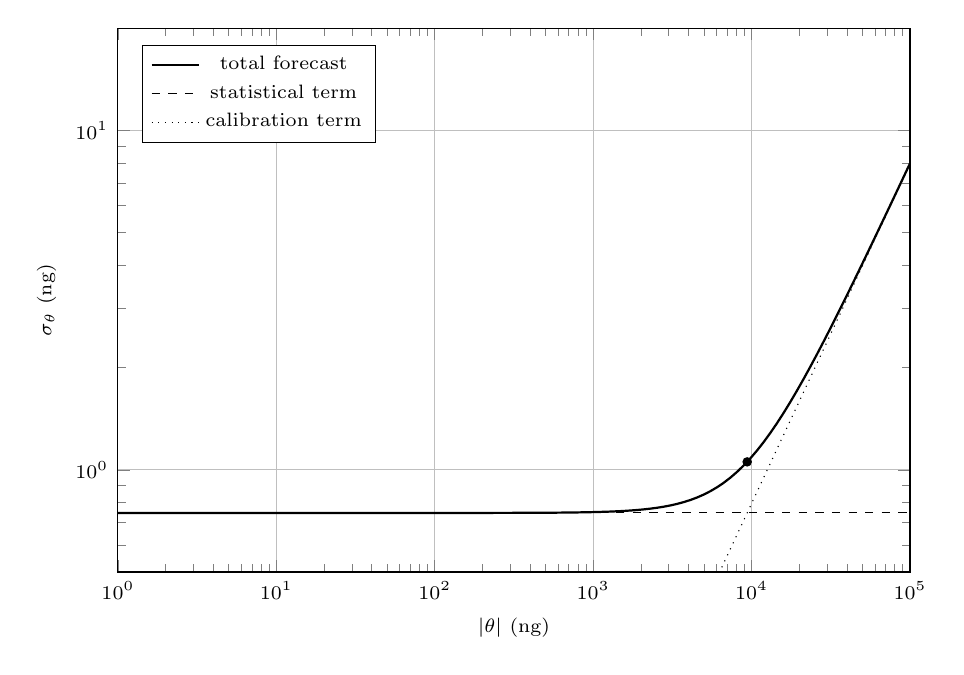
\begin{tikzpicture}
\begin{loglogaxis}[
width=0.96\columnwidth,height=0.70\columnwidth,
xlabel={$|\theta|$ (ng)},ylabel={$\sigma_\theta$ (ng)},
xmin=1,xmax=100000,ymin=0.5,ymax=20,
grid=major,legend style={font=\scriptsize,at={(0.03,0.97)},anchor=north west},
tick label style={font=\scriptsize},label style={font=\scriptsize}]
\addplot[domain=1:100000,samples=120,thick] {sqrt(0.746604^2+(x*7.95629794e-5)^2)};
\addlegendentry{total forecast}
\addplot[domain=1:100000,samples=2,dashed] {0.746604};
\addlegendentry{statistical term}
\addplot[domain=1:100000,samples=2,dotted] {x*7.95629794e-5};
\addlegendentry{calibration term}
\addplot[only marks,mark=*,mark size=1.5pt] coordinates {(9383.82,1.05557)};
\end{loglogaxis}
\end{tikzpicture}
\caption{One-hour statistical/calibration resource boundary for the declared differential-chirp reference architecture. The total curve follows Eq.~\eqref{eq:floorlaw}. The crossing of the two contributions occurs at $|\theta|\simeq9.38\,\mu g$. This is a design forecast, not an observed signal amplitude.}
\label{fig:crossover}
\end{figure}

The chirp-reference PASS has strict boundaries. The differential chirp must be independently measured against calibrated time/frequency standards; the mapping from commanded electronics to the actual Raman difference-frequency chirp must be verified; and $k_{\rm eff}$ must be tied to the actual optical frequencies and beam geometry. A merely commanded but unmeasured chirp is not certified reference metrology.
